%%================================================
%% Filename: chap04.tex
%% Encoding: UTF-8
%% Author: Yuan Xiaoshuai - yxshuai@gmail.com
%% Created: 2012-04-28 00:15
%% Last modified: 2019-11-06 17:39
%%================================================
\chapter{基于特征选择优化的 ResNet-BiGRU 分类检测模型}

\label{cha:ResNet-BiGRU}

在现代网络安全领域,快速准确地检测潜在攻击的能力至关重要。
但是,我们面临的挑战在于,传统的攻击检测方法往往依赖于预先定义的特征集,这可能导致对新型攻击的检测能力不足,因为它们无法适应不断变化的攻击模式。
另外,实际的流量数据有着海量高维的特点,然而常规的算法通常不会针对这种特点进行调整适应,往往结果是生成的模型在实际部署中准确率低、误报率高。
因此,为了能够解决这种概念漂移问题和能够有效挖掘复杂网络数据的深层特征以达到更高的检测精度,我们引入了基于特征选择优化的 ResNet-BiGRU 分类检测模型。
图~\ref{fig:attack_detecion_model}~描述了我们的检测模型的工作原理和流程。
\begin{figure}[htbp]
  \centering
  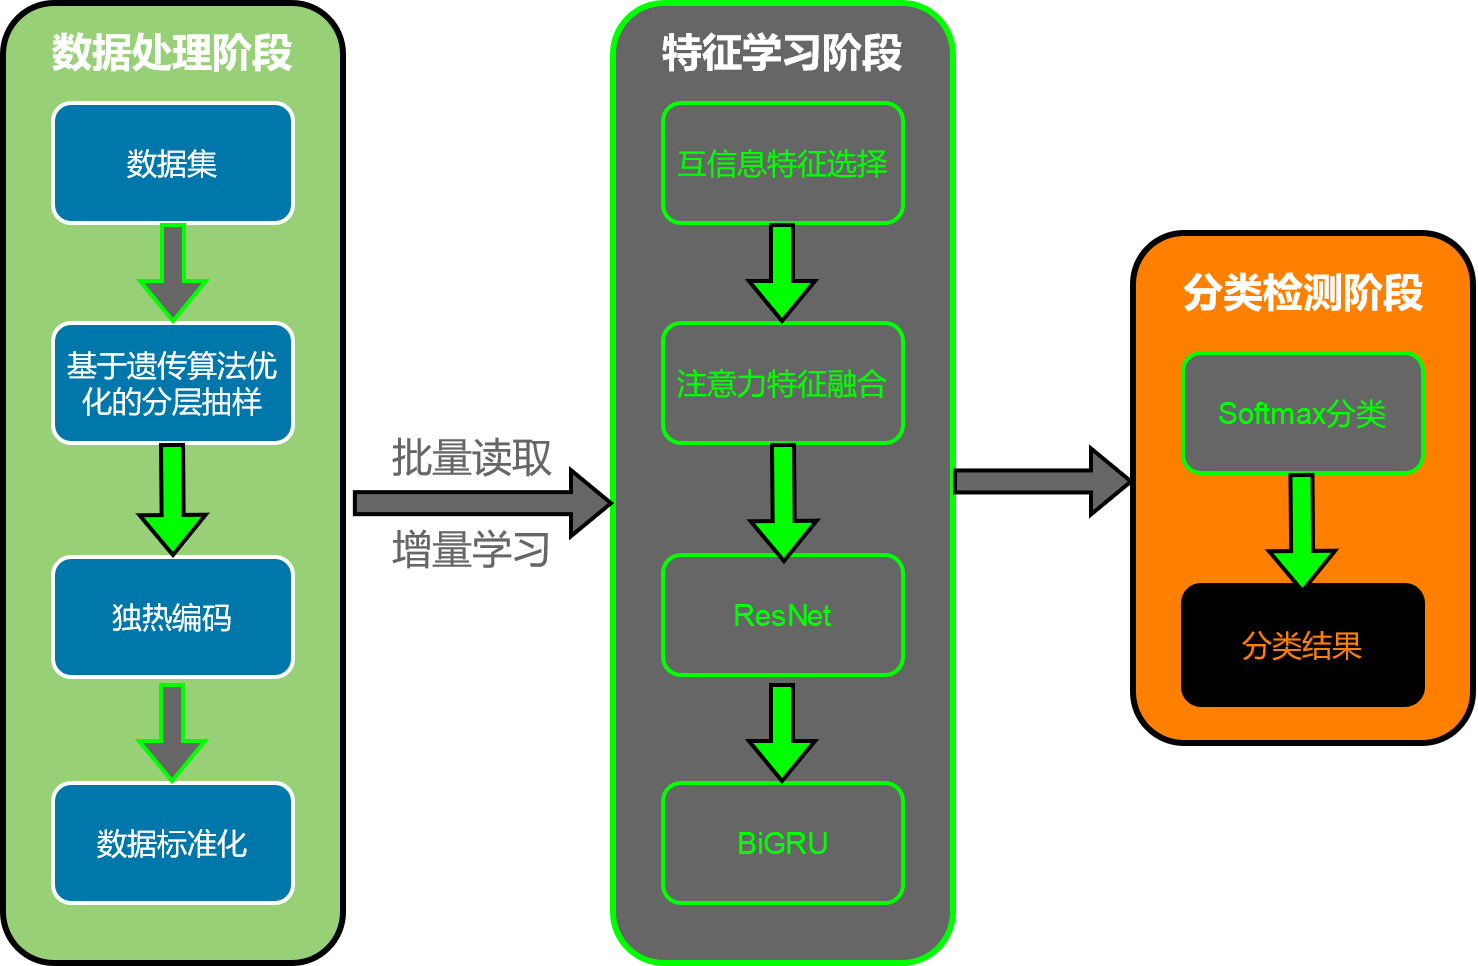
\includegraphics[width = 0.8\textwidth]{ourmodel.drawio.png}
  \caption{基于特征选择优化的 ResNet-BiGRU 分类检测模型}
  \label{fig:attack_detecion_model}
\end{figure}


模型首先采用遗传算法对分层抽样过程进行优化,保证训练集的质量;
之后利用互信息冗余算法进行特征降维来提高算法效率减少过拟合的风险;
训练采用增量学习的方式适应不断变化的攻击模式,减少对数据集的依赖性;
最后利用ResNet-BiGRU的优势来解决深度网络中的梯度消失问题、捕捉时间序列数据中的长期依赖关系,从而挖掘复杂网络数据的深层特征,提高检测精度和准确率。
接下来,我们将详细地从实验数据集、数据集预处理、模型具体结构设计、实验设置、实验结果逐步展开介绍。

\section{实验数据集}
\subsection{NSL-KDD数据集\cite{revathi2013detailed}}
KDD Cup 99数据集\cite{tavallaee2009detailed}曾长期被视为网络入侵检测研究的标准化数据集。
然而,该数据集存在一些显著的局限性,例如庞大的数据量和大量的冗余记录,这些因素共同导致了模型训练和测试的效率低下。
为了解决这些问题并提高研究效率,NSL-KDD数据集应运而生,它在网络安全领域得到了广泛的应用和认可。


NSL-KDD数据集的设计考虑到了消除冗余性、改善平衡性、增加多样性和扩展适用性。
通过从原始的KDD Cup 99数据集中移除冗余记录,NSL-KDD显著减少了数据量,从而使得模型和算法能够在较短的时间内完成训练,同时降低了因数据冗余可能引入的偏差风险。
尽管NSL-KDD并未完全解决数据类别不平衡的问题,但相较于其前身,它在一定程度上减轻了这一问题,为研究人员提供了一个更加平衡的数据环境。


NSL-KDD数据集由41个特征组成,整体包括八个文件,分成四组数据,每组提供了两种格式:文本(.txt)和属性关系文件格式(.arff)。
这些文件的详细描述如下表~\ref{tab:NSLKDDFile}~。
\begin{table}[htbp]
  \caption{NSL-KDD数据集各文件介绍}
  \label{tab:NSLKDDFile}
  \begin{tabularx}{\textwidth}{cXc}
    \toprule
    \textbf{文件名} & \textbf{描述} & \textbf{记录总数}\\
  \midrule
    KDDTrain+.ARFF & 完整的NSL-KDD训练集以二进制标签的ARFF格式提供 &125973\\
    KDDTrain+.TXT & 完整的NSL-KDD训练集,包括攻击类型标签和难度级别,以CSV格式提供&125973\\
    KDDTrain+20Percent.ARFF & KDDTrain+.arff文件的20\%子集&25192\\
    KDDTrain+20Percent.TXT & KDDTrain+.txt文件的20\%子集 &25192\\
    KDDTest+.ARFF & 完整的NSL-KDD测试集以二进制标签的ARFF格式提供 &22544\\
    KDDTest+.TXT & 完整的NSL-KDD测试集,包括攻击类型标签和难度级别,以CSV格式提供 & 22544\\
    KDDTest-21.ARFF & 不包含难度级别为21的记录的KDDTest+.arff文件的子集 &11850\\
    KDDTest-21.TXT & 不包含难度级别为21的记录的KDDTest+.txt文件的子集&11850 \\
  \bottomrule
  \end{tabularx}
\end{table}

NSL-KDD数据集中包含的攻击流量可分为拒绝服务攻击(DoS)、远程到本地攻击(R2L)、用户到根攻击(U2R)以及探测攻击(Probe)共四种类别。
如表~\ref{tab:attack_class}~所示,这四种类别又可细分为39种子类型。
表~\ref{tab:kdd_distribution}~则展示四种类别的攻击流量与正常流量在数据集中的分布占比。
图~\ref{fig:kddtraindistribution}~、~\ref{fig:kddtestdistribution}~分别是完整训练集与测试集中各种流量分布占比饼状图。


通过以上图表可知数据集中不同攻击类型的数据分布不均衡,特别是U2R和R2L攻击类型的样本数量远少于其他类型。
这种不平衡分布对于训练入侵检测系统模型来说是一个挑战,因为模型可能会在较多样本的攻击类型上表现更好,而在样本较少的攻击类型上表现不佳。
此外,从KDDTrain+到KDDTest+,攻击类型的分布变化表明,测试集可能代表了与训练集不同的攻击环境,这要求模型具备良好的泛化能力,以适应不同的攻击行为和模式。


\begin{table}[htbp]
  \caption{NSL-KDD数据集中每种攻击的不同子类的细分}
  \label{tab:attack_class}
  \begin{tabularx}{\textwidth}{@{}ccX@{}}
  \toprule
    \multicolumn{1}{c}{\textbf{种类}} & \multicolumn{1}{c}{\textbf{数量}} & \multicolumn{1}{c}{\textbf{子类}}\\
  \midrule
    DoS & 11 & apache2, back, land, neptune, mailbomb, pod, processtable, smurf, teardrop, dupstorm, worm\\
    Probe & 6 & ipsweep, mscan, nmap, portsweep, saint, satan\\
    U2R & 7 & buffer\_overflow, loadmodule, perl, ps, rootkit, sqlattack, xterm\\
    R2L & 15 & ftp\_write, guess\_passwd, httptunnel, imap, multihop, named, phf, sendmail, snmpattack, spy, snmpguess, warezclient, warezmaster, xlock, xsnoop\\
  \bottomrule
  \end{tabularx}
\end{table}

\begin{table}[htbp]
  \caption{每种攻击类型的数据分布}
  \label{tab:kdd_distribution}
  \centering
  \begin{tabular}{ccccccc}
  \toprule
  \textbf{数据集} & \textbf{总数} & \textbf{Normal} & \textbf{DoS} & \textbf{Probe} & \textbf{R2L} & \textbf{U2R}\\
  \midrule
  \multirow{2}{*}{KDDTrain+} & \multirow{2}{*}{125973} & 67343 & 45927 & 11656 & 995  & 52   \\
                             &                          &53.46\%& 36.46\% & 9.25\%&0.79\%&0.04\%\\
  \multirow{2}{*}{KDDTest+} & \multirow{2}{*}{22544} & 9711 & 7636 & 2423 & 2574 & 200\\
                            &                           & 43.08\% & 33.87\%& 10.74\%& 11.42\%&0.89\%\\
  \multirow{2}{*}{KDDTrain+20\%} & \multirow{2}{*}{25192} & 13449 & 9234 & 2289 & 209 & 11\\
                                 &                      & 53.39\% & 36.65\%& 9.09\%& 0.83\%&0.04\%\\
  \bottomrule
  \end{tabular}
\end{table}

  \begin{figure}[htbp]
    \centering
    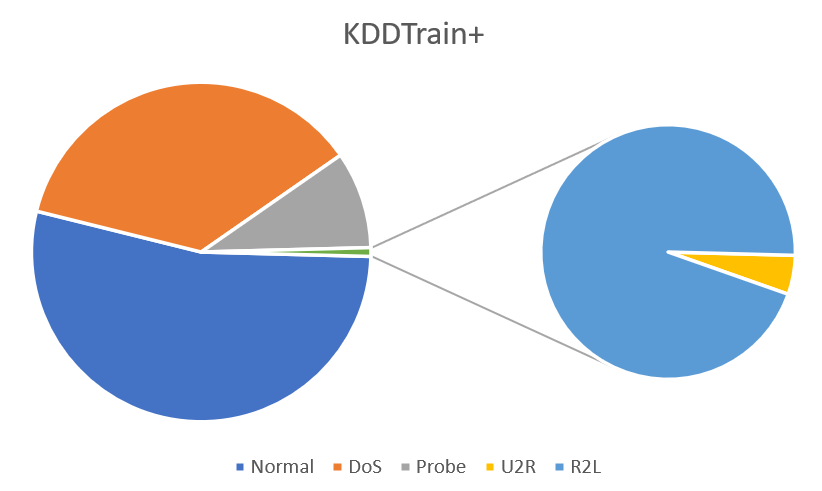
\includegraphics[width = 0.8\textwidth]{kddtraindistribution.png}
    \caption{NSL-KDD完整训练集分类占比饼状图}
    \label{fig:kddtraindistribution}
  \end{figure}

  \begin{figure}[htbp]
    \centering
    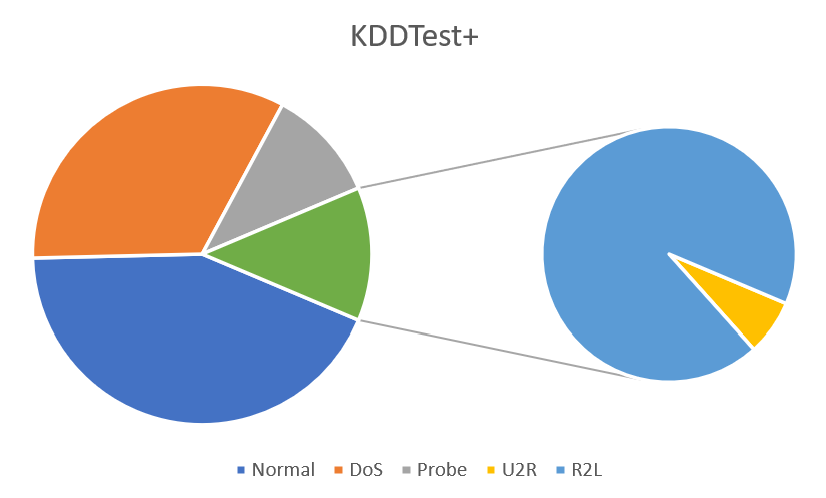
\includegraphics[width = 0.8\textwidth]{kddtestdistribution.png}
    \caption{NSL-KDD完整测试集分类占比饼状图}
    \label{fig:kddtestdistribution}
  \end{figure}

\section{数据预处理}
数据预处理是深度学习或机器学习一个至关重要的步骤,
进行数据预处理的目的是制作出一个干净、标准化、均衡的数据集,为特征学习和后续的模型训练打下坚实的基础。
正确的数据预处理策略可以显著提高模型的性能,加快训练速度,并提高模型在未见数据上的泛化能力。
本文在数据预处理阶段采取了综合性的方法论,旨在优化模型的学习效率和性能。\par

首先,对训练集和测试集执行特征编码,以便将分类数据转换为模型可处理的格式。
随后,本研究针对原始数据集及特征编码过程中可能产生的缺失值进行了细致的处理,确保数据的完整性。
在完成上述步骤后,进一步通过特征选择技术降低数据维度,这一步骤旨在剔除冗余或不相关的特征,从而提高模型训练的效率并可能提升模型的泛化能力。
此外,对特征选择后的数据进行标准化处理,确保所有特征都在相同的尺度上,进一步促进模型学习。
鉴于本文采用增量学习策略以及数据集呈现显著的不平衡性,本文将会对数据集进行分层抽样优化,以期在训练过程中实现更为均衡的类别表示和提升模型对少数类的识别能力。\par

图~\ref{fig:dataprocess}~概括性地展示了整个数据预处理和模型训练的流程。
本节接下来的部分将对这一流程中的关键步骤进行详细阐述,以便于读者深入理解本研究采取的方法论及其背后的逻辑。
\begin{figure}[htbp]
  \centering
  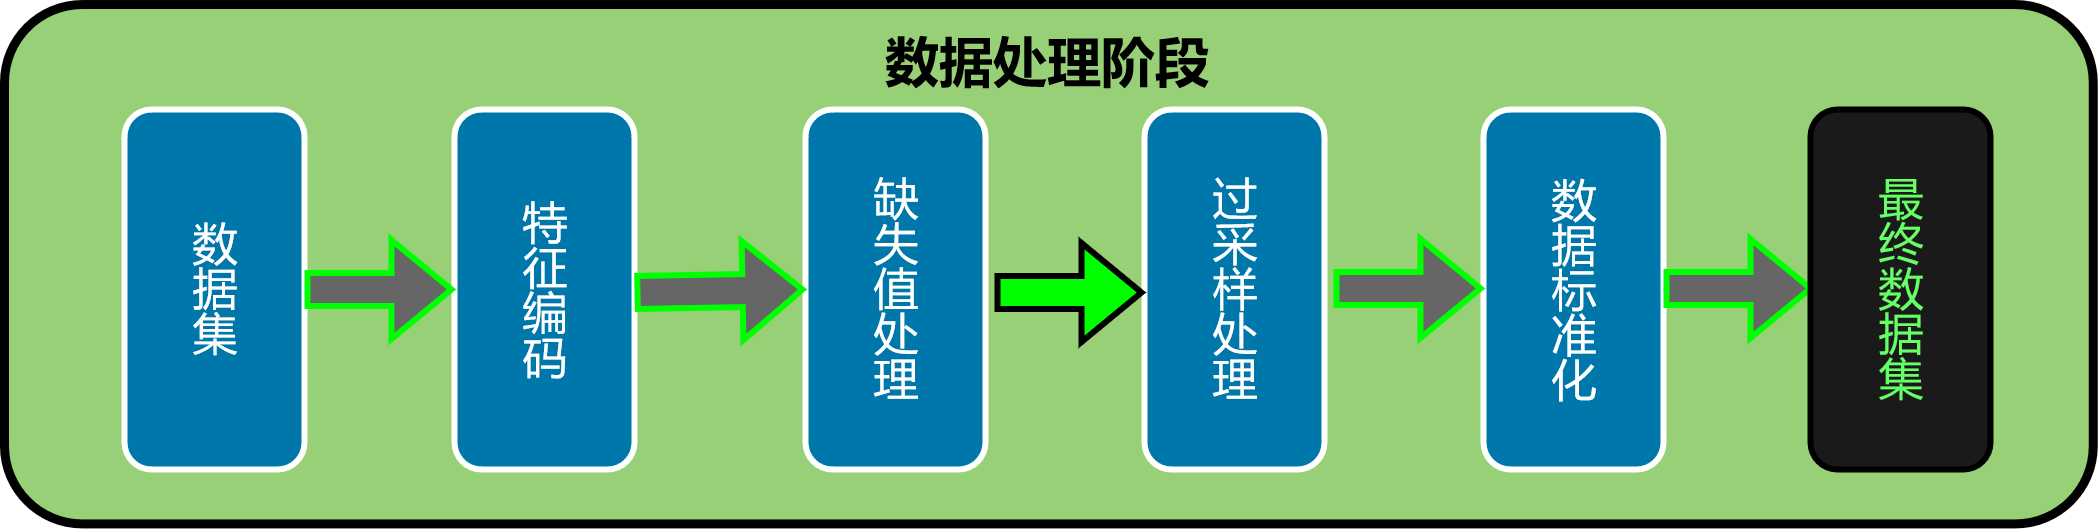
\includegraphics[width = 0.8\textwidth]{dataprocess.drawio.png}
  \caption{数据集预处理流程图}
  \label{fig:dataprocess}
\end{figure}

\subsection{特征编码}
\begin{table}[htbp]
  \caption{One-hot编码算法实现}
  \label{tab:onehot}
  \centering
  \begin{tabularx}{1.0\textwidth}{cl}
  \toprule
  \multicolumn{2}{l}{\textbf{one-hot编码算法}}\\
  \midrule
  \multicolumn{2}{l}{\textbf{输入}: 数据集 $D$,其中包含数值型和分类型列} \\ 
  \multicolumn{2}{l}{\textbf{输出}: 经过One-hot编码的数据集 $D'$} \\
  1& 初始化一个空的数据集 $D'$ \\
  2& \textbf{for} 每一列 $col$ \textbf{in} $D$: \\
  3&\quad \textbf{if} $col$ 是分类型: \\
  4&\quad\quad $unique\_values$ = 获取 $col$ 的所有唯一值 \\
  5&\quad\quad \textbf{for} 每一个值 $val$ \textbf{in} $unique\_values$: \\
  6&\quad\quad\quad 创建一个新列 $new\_col$,名称为 ``$col\_val$''\\
  7&\quad\quad\quad \textbf{for} 每一行 $row$ \textbf{in} $D$: \\
  8&\quad\quad\quad\quad \textbf{if} $row[col] == val$: \\
  9&\quad\quad\quad\quad\quad 在 $D'[new\_col]$ 中填充 1 \\
  10&\quad\quad\quad\quad \textbf{else}: \\
  11&\quad\quad\quad\quad\quad 在 $D'[new\_col]$ 中填充 0 \\
  12&\quad \textbf{else}: \\
  13&\quad\quad 将 $col$ 直接复制到 $D'$ 中 \\
  14&\textbf{return} $D'$ \\ 
  \bottomrule
  \end{tabularx}
  \end{table}
特征编码是一种数据预处理方法,用于将原始数据转换为机器学习算法能够理解和处理的格式。
这个过程对于提高模型的性能和准确性至关重要,因为大多数机器学习算法预期输入数据为数值型,而原始数据往往包括各种类型,如文本、日期或分类数据。
特征编码操作的目的便是将非数值特征转换为数值形式,使算法能够对这些数据进行计算。
因为我们的流量数据集中也存在着许多非数值类型的特征,所以我们这里也需要对数据集进行特征编码,将非数值类型转为数值类型。\par

One-Hot 编码是一种特殊且广泛使用的特征编码方法,它易于理解和实现,非常适用于处理具有有限类别的分类数据。
因此我们这里将选用,one-hot编码方法进行特征编码。
这种编码方法通过为每个类别创建一个新的二进制列来工作。
对于每个数据点,它所属的类别的列被标记为1,而所有其他列被标记为0。
表~\ref{tab:onehot}~是本文采用one-hot编码对数据集进行特征编码的具体算法。


\subsection{特征选择阶段}
在数据预处理阶段,特征选择扮演了至关重要的角色,其核心目标是从原始数据集中挑选出对预测目标变量有显著贡献的特征。
这一过程对于降低模型复杂度、加快训练速度以及提升模型性能至关重要,原因在于它能有效去除数据中的噪声和不相关特征。
通过实施有效的特征选择,不仅可以减轻过拟合的风险,还能增强模型对新数据的泛化能力。

为了实现这一目标,本研究采用遗传算法对特征选择过程进行优化。
遗传算法,作为一种启发式搜索算法,受到生物进化机制的启发,通过模拟自然选择、遗传、变异等过程来解决优化问题。
本文在第~\ref{eq:GA}~章已详细介绍了遗传算法的理论基础,因此此处不再展开,而是直接进入具体的实施细节。\par

(1) 遗传算法的选择\par
遗传算法的种类以及策略多种多样,在这里我们选择采用稳态遗传算法(Steady State Genetic Algorithm, SSGA)作为优化策略。
与传统的遗传算法相比,稳态遗传算法的特点在于每次迭代只替换种群中的一小部分个体,而不是进行全种群的更新。
这种方法的优势在于绝大多数个体在迭代过程中保持不变,从而避免了每次迭代都进行完整的种群更换。\par

考虑到本文中个体适应度评估的复杂性——每个个体的评估需要经过完整的模型训练及性能评估过程——采用标准遗传算法(即采用完全生成替换策略的遗传算法,其中每次迭代都替换整个种群)将显著增加计算负担,并可能不利于优良基因的保留。
相反,稳态遗传算法通过每次只替换部分种群的策略,不仅大幅度降低了计算量,而且有助于保持种群中的优秀个体。
这种策略的实施有助于加速算法的收敛过程,并且,通过有效地保留高质量的解,稳态遗传算法能够在全局搜索和局部搜索之间取得更好的平衡,从而提高发现全局最优解的可能性。

(2) 染色体编码\par

遗传算法的每个个体(或称为“染色体”)代表一种可能的特征子集选择方案,其中包含了样本每个特征的选择情况。
本文将利用二进制编码的方案对特征进行选择,染色体种的每一个基因(即:1bit位)位对应样本的一个特征位。
基因值代表该特征位的选择情况,例如一条染色体的前5位基因分别为{0,1,0,1,1},则代表样本中第二位以及第四、五位的特征要被选择,而第一、三位则被忽略掉。
下表~\ref{tab:Ga_code}~是这一过程的对应情况。
在本方案中,由于样本的特征数量有限,一条染色体的基因数量可以由特征数量决定,通过这样的方法能够选出一组最优特征子集。

在遗传算法中,每个个体(也称作“染色体”)代表了一种潜在的特征选择方案,通过对样本中每个特征是否被选中的表示来体现。
为了实现这一表示,本文采用了二进制编码策略,其中染色体上的每个基因(即1位二进制数)对应于样本的一个特征。
在此方案下,染色体的基因数量直接对应于特征的总数。
基因的值(0或1)指示相应特征是否被选中:1表示选择该特征,而0表示忽略该特征。
例如,假设某个染色体的前五个基因位为{0,1,0,1,1},这表示选择样本中的第二、第四和第五个特征,而第一和第三个特征则被排除。
表~\ref{tab:Ga_code}~是这一过程的对应情况。

\begin{table}
  \caption{遗传算法编码方案}
  \label{tab:Ga_code}
  \centering
  \begin{tabular}{cccccc}
    \toprule
    \textbf{编码值(基因)}&0&1&0&1&1\\
    \midrule
    \textbf{特征}&duration&protocol\_type&service&flag&src\_bytes\\
    \textbf{选择}&$\times$&\checked&$\times$&\checked&\checked\\
    \bottomrule
  \end{tabular}
\end{table}


\begin{table}[htbp]
  \caption{遗传算法实现}
  \label{tab:genetic_algorithm}
  \centering
  \begin{tabularx}{1.0\textwidth}{cl}
  \toprule
  \multicolumn{2}{l}{\textbf{遗传算法}}\\
  \midrule
  \multicolumn{2}{l}{\textbf{输入}: 种群大小 $P$,基因数量 $G$,代数 $N$,变异率 $M$} \\
  \multicolumn{2}{l}{\textbf{输出}: 适应度最高的染色体} \\
  1& 初始化种群 $pop$ \\
  2& \textbf{for} 每一代 \textbf{in} $N$: \\
  3&\quad 选择两个父代 $p1$ 和 $p2$ \\
  4&\quad 生成两个后代 $c1$ 和 $c2$ 通过 $crossover(p1, p2)$ \\
  5&\quad 对 $c1$ 和 $c2$ 进行 $mutate$ 操作 \\
  6&\quad 将 $c1$ 和 $c2$ 加入到 $pop$ 中 \\
  7&\quad 计算种群中每个个体的适应度: \\
  7&\quad\quad\quad\quad 根据染色体编码进行特征选择 \\
  7&\quad\quad\quad\quad 训练模型 \\
  7&\quad\quad\quad\quad 评估模型,取得适应度\\
  8&\quad 根据适应度计算每个个体的淘汰概率 \\
  9&\quad 淘汰两个适应度最低的个体 \\
  10& \textbf{return} 适应度最高的染色体 \\
  \bottomrule
  \end{tabularx}
\end{table}
(3) 适应度评估\par
本文将会把数据集分为训练集和验证集,根据染色体中的特征选择情况对数据集进行处理并对所有待提升的模型进行训练。
模型得出的验证结果将作为适应度评估值。并使用weighted avg f1-score(公式~\ref{eq:val_score5}~)作为评价标准。
这里没有选用accuracy\_score而选用weighted avg f1-score的原因是
accuracy\_score 虽然简单直观,易于理解但在在类别不平衡的数据集中可能会产生误导。
例如,如果一个类占95\%的样本,模型总是预测这个主要类别,那么准确率可能达到95\%,但这并不意味着模型具有良好的性能。
而weighted avg f1-score 计算精确度(precision)和召回率(recall)的调和平均,对于每个类别分别计算F1分数,并根据每个类别的样本数(support)进行加权平均。
因此weighted avg f1-score能够综合考虑精确度、召回率以及样本类别数量,即使数据集处于不平衡的情况,也能很好地反映模型的性能。\par

(4) 初始群体生成及迭代次数\par
为了确保算法能够充分探索解空间并增加解的多样性,我们特别注重初代种群的广泛性和迭代过程的深入性。
基于此目的,初始种群规模被设定为1,000个个体。
这一较大的初始种群规模有助于覆盖更广泛的解空间,从而提高找到全局最优解的概率。
同时,为了充分优化解并观察算法的收敛行为,设置了10,000次的迭代次数,以便于算法有足够的时间逐步改进解,并最终接近最优解。\par



(5) 选择、交叉和变异\par
对于选择策略,本文采用轮盘赌选择法,该方法根据个体适应度相对于总体适应度的比例来分配选择概率。
这种方法的优势在于能够有效保证高适应度个体被优先选择,从而引导种群朝着更优解空间方向进化。
在交叉操作方面,为了降低计算的复杂度,本文选择了单点交叉方法。
对于变异策略,本研究设置了0.1的固定概率对新生成的个体中的所有基因进行变异。

表~\ref{tab:genetic_algorithm}~是我们遗传算法实现的伪代码。



\section{特征学习阶段}

\section{实验评估与分析}
\subsection{实验环境}
为了评估本文所提方案的有效性,本文将利用python语言来实现以上流程,并选用表~\ref{tab:env_setting}~中的配置来进行实验。
\begin{table}[htbp]
  \caption{实验设备配置}
  \label{tab:env_setting}
  \centering
  \begin{tabular}{ccc}
    \toprule
    \textbf{环境类别} & \textbf{设备项目} & \textbf{项目参数}\\
    \midrule
    \multirow{6}{*}{硬件环境}& CPU型号 & Intel(R) Core(TM) i7-11800H\\
                            & CPU规格 & 8核16线程@2.30GHz\\
                            & GPU型号 & NVIDIA GeForce RTX 3060 Laptop GPU\\
                            & 内存大小& 16.0 GB\\
                            & 硬盘类型& SSD\\
                            & 硬盘大小& 1TB\\
                            \hline
    \multirow{3}{*}{软件环境}&操作系统&Windows 11\\
                            &开发语言&Python 3.11.7\\
                            &编辑器 &Visual Studio Code\\                       
    \bottomrule
  \end{tabular}
\end{table}

\subsection{评估指标}
本文主要使用准确度 (Accuracy)、精确度 (Precision)、召回率 (Recall)、F1 分数 (F1 Score)、宏平均 F1 分数 (Macro Averaged F1 Score)、
ROC-AUC 分数 (ROC-AUC Score)、混淆矩阵 (Confusion Matrix)这7个评价指标对我们的方案进行全方位的评估。以下是这7个指标的简单介绍。\par
(1) 准确度\par
表示模型正确预测的比例,是所有正确预测的数量除以总预测数量。
\begin{equation}
  \label{eq:val_score1}
  Accuracy = \frac{Number of Correct Predictions}{Total Number of Predictions} = \frac{TP + TN}{TP + TN + FP + FN}
\end{equation}

(2) 精确度\par
简称精度,也称为查准率,是所有模型预测为正类的样本中,实际为正类的比例。
\begin{equation}
  \label{eq:val_score2}
  Precision = \frac{TP}{TP + FP}
\end{equation}

(3) 召回率\par
召回率,也称为真正率、查补率,是模型正确识别为正类的样本占所有实际正类样本的比例。
\begin{equation}
  \label{eq:val_score3} 
  Recall = \frac{TP}{TP + FN}
\end{equation}

(4) F1 分数\par
F1 分数是精确度和召回率的调和平均,用于衡量模型的精确度和召回率的平衡程度。
\begin{equation}
  \label{eq:val_score4}
  F1 = 2 \times \frac{Precision \times Recall}{Precision + Recall} = \frac{2TP}{2TP + FP + FN}
\end{equation}

(5) 加权平均 F1 分数\par
加权平均F1分数是一种性能评估指标,通过根据每个类别的样本量对其F1分数进行加权平均,以反映所有类别的整体性能。
每个类别的重要性通过其在数据集中的相对比例来确定。

\begin{equation}
  \label{eq:val_score5}
  F1_{weighted} = \sum\limits_{i=1}^{N} w_i \cdot F1_i
\end{equation}
\begin{flushleft}
  \renewcommand\arraystretch{1.25}
  \begin{tabularx}{\textwidth}{@{}>{\normalsize\rm}l@{\quad}>{\normalsize\rm}l@{——}>{\normalsize\rm}X@{}}
  式中& $\symbf{F1_{weighted}}$ &加权平均F1分数;\\
  &  $\symbf{N}$&类别总数;\\
  &  $\symbf{F1_i}$ &第$i$个类别的F1分数\\
  &  $\symbf{w_i}$ & 第$i$个类别的权重,通常由该类别的样本数量占总样本数量的比例确定。\\
  \end{tabularx}\vspace{.5ex}%TODO : 注释内容自动转页接排
  \end{flushleft}

(6) 混淆矩阵\par
混淆矩阵是一种特定的表格布局,用于可视化模型性能,显示实际类别与模型预测类别之间的关系。
\begin{equation}
  \label{eq:val_score6}
  Confusion Matrix = \begin{bmatrix} TP & FP \\ FN & TN \end{bmatrix}
\end{equation}

(7) ROC-AUC 分数\par
ROC-AUC 分数是接收者操作特征(ROC)曲线下面积的度量,用于评估分类器的预测能力。
\begin{equation}
  \label{eq:val_score7}
  AUC = \int_{0}^{1} TPR(FPR) \, d(FPR)
\end{equation}

以上七个式\ref{eq:val_score1}、\ref{eq:val_score2}、\ref{eq:val_score3}、\ref{eq:val_score4}、\ref{eq:val_score5}、\ref{eq:val_score6}、\ref{eq:val_score7}中,
  $TP$(True Positives)表示正确地将正类预测为正类;
  $TN$(True Negatives)表示正确地将负类预测为负类;
  $FP$(False Positives)表示错误地将负类预测为正类;
  $FN$(False Negatives)表示错误地将正类预测为负类。


% 在~\LaTeX~中应用最多的图片格式是~EPS(Encapsulated PostScript)格式,它是一种
% 专用的打印机描述语言,常用于印刷或打印输出。EPS~格式图片可通过多种方式生成,
% 如果使用命令行界面,则可以用 ImageMagick,可将其它格式图片转换为~EPS~格式图
% 片,同时还可以锐化图片,使图片的局部清晰一些。

% ImageMagick 包含多个命令行程序,其中最常用的是 \texttt{convert}。
% \begin{shell}
% convert [可选参数] 原文件名.原扩展名 新文件名.eps
% \end{shell}

% 除此之外,一些文字处理软件和科学计算软件也支持生成~EPS~格式的文件,可用“另存
% 为”功能查看某款软件是否能够将图片以~EPS~格式的形式保存。

% \subsection{插入单幅图形}

% 插图通常需要占据大块空白,所以在文字处理软件中用户经常需要调整插图的位置。
% \LaTeX~有一个 \texttt{figure} 环境可以自动完成这样的任务,这种自动调整位置的环
% 境称作浮动环境(float),之后还会介绍表格浮动环境。

% 单张图片插入形式如图~\ref{fig:golfer}~所示。
% \begin{figure}[htbp]
% \centering
% \includegraphics[width = 0.3\textwidth]{golfer}
% \caption{打高尔夫球的人}
% \label{fig:golfer}
% \end{figure}

% \begin{latex}
% \begin{figure}[htbp]
% \centering
% \includegraphics[width=0.3\textwidth]{golfer}
% \caption{打高尔夫球的人}
% \label{fig:golfer}%应放在\caption{}之后,否则引用时指向的是前一个插图
% \end{figure}
% \end{latex}

% 上述代码中,\verb|[htbp]| 选项用来指定插图排版的理想位置,这几个字母分别代表
% ~here、top、bottom、float page,也就是固定位置、页顶、页尾、单独的浮动页。可
% 以使用这几个字母的任意组合,一般不推荐单独使用 \verb|[h]|。如果要强制固定浮动
% 图形的位置,还可以用 \textbf{float} 宏包的 \verb|[H]| 选项。

% \subsection{插入多幅图形}

% \subsubsection*{并排摆放,共享标题}

% 当我们需要两幅图片并排摆放,并共享标题时,可以在 \texttt{figure} 环境中使用两个
% \begin{latex}
% \includegraphics{}
% \end{latex}
% 命令,如图~\ref{fig:fanqingfuming}~所示。

% \begin{latex}
% \begin{figure}[htbp]
% \centering
% \includegraphics[width=0.3\textwidth]{qingming}
% \hspace{36pt}
% \includegraphics[width=0.3\textwidth]{fanfu}
% \caption{反清复明}
% \label{fig:fanqingmuming}
% \end{figure}
% \end{latex}

% \begin{figure}[htbp]
% \centering
% \includegraphics[width=0.3\textwidth]{qingming}
% \hspace{36pt}
% \includegraphics[width=0.3\textwidth]{fanfu}
% \caption{反清复明}
% \label{fig:fanqingfuming}
% \end{figure}

% \subsubsection*{并排摆放,各有标题}

% 如果想要两幅并排的图片各有自己的标题,可以在 \texttt{figure} 环境中使用两个
%  \texttt{minipage} 环境,每个环境里插入一个图,如图~\ref{fig:qingming}~和
% ~\ref{fig:fanfu}~所示。

% \begin{latex}
% \begin{figure}[htbp]
% \centering
% \begin{minipage}[t]{0.3\textwidth}
%     \centering
%     \includegraphics[width=\textwidth]{qingming}
%     \caption{清明}
%     \label{fig:qingming}
% \end{minipage}
% \hspace{36pt}
% \begin{minipage}[t]{0.3\textwidth}
%     \centering
%     \includegraphics[width=\textwidth]{fanfu}
%     \caption{反复}
%     \label{fig:fanfu}
% \end{minipage}
% \end{figure}
% \end{latex}

% \begin{figure}[htbp]
% \centering
% \begin{minipage}[t]{0.3\textwidth}
%     \centering
%     \includegraphics[width=\textwidth]{qingming}
%     \caption{清明}
%     \label{fig:qingming}
% \end{minipage}
% \hspace{36pt}
% \begin{minipage}[t]{0.3\textwidth}
%     \centering
%     \includegraphics[width=\textwidth]{fanfu}
%     \caption{反复}
%     \label{fig:fanfu}
% \end{minipage}
% \end{figure}

% \subsubsection*{并排摆放,共享标题,各有子标题}

% 如果想要两幅并排的图片共享一个标题,并各有自己的子标题,可以使用
% \textbf{subcaption} 宏包提供的
% \begin{latex}
% \subcaptionbox{<title>}[<width>]{<insertfigure>}
% \end{latex}
% 命令,如图~\ref{fig:subfig_a}~和~\ref{fig:subfig_b}~所示。

% \begin{latex}
% \begin{figure}[htbp]
%   \centering
%   \subcaptionbox{清明\label{fig:subfig_a}}[0.3\textwidth]{
%       \includegraphics[width=0.3\textwidth]{qingming}
%   }
%   \hspace{36pt}
%   \subcaptionbox{反复\label{fig:subfig_b}}[0.3\textwidth]{
%       \includegraphics[width=0.3\textwidth]{fanfu}
%   }
%   \caption{反清复明}
% \end{figure}
% \end{latex}

% 每个子图可以有各自的引用,就象这个样子:\ref{fig:subfig_a}、
% \ref{fig:subfig_b}。

% \begin{figure}[htbp]
% \centering
% \subcaptionbox{清明\label{fig:subfig_a}}[0.3\textwidth]{
%     \includegraphics[width=0.3\textwidth]{qingming}
% }
% \hspace{36pt}
% \subcaptionbox{反复\label{fig:subfig_b}}[0.3\textwidth]{
%     \includegraphics[width=0.3\textwidth]{fanfu}
% }
% \caption{反清复明}
% \end{figure}

% \section{表格示例}
% \label{sec:table}

% 模板中关于表格的宏包有四个:\textbf{tabularx}、\textbf{multirow}、
% \textbf{longtable} 和\textbf{booktabs}。长表格还可以用\textbf{supertabular},
% 可以方便地在表格下方加入脚注。

% \subsection{普通表格的绘制方法}

% \texttt{table} 环境是一个将表格嵌入文本的浮动环境,其标题和交叉引用的用法类似
% 于上一节提到的图形浮动环境 \texttt{figure}。该环境提供了最简单的表格功能,常用命令如下
% \begin{latex}
% \hline % 横线
% |      % 竖线
% &      % 分列
% \\     % 换行
% l c r  % 横向居中、居左、居右对齐  
% \end{latex}

% 科技文献中常使用三线表格,因此需要调用 \textbf{booktabs} 宏包,三条横线就分别
% 用
% \begin{latex}
% \toprule
% \midrule
% \bottomrule
% \end{latex}
% 等命令表示。其标准格式如表~\ref{table1}~所示。

% \begin{table}[htbp]
% \caption{文献类型和标识代码}
% \label{table1}
% \centering
% \begin{tabular}{cccc}
% \toprule
% 文献类型 & 标识代码 & 文献类型 & 标识代码\\
% \midrule
% 普通图书 & M &  会议录 & C\\
% 汇编 & G & 报纸 & N\\
% 期刊 & J & 学位论文 & D\\
% 报告 & R & 标准 & S\\
% 专利 & P & 数据库 & DB\\
% 计算机程序 & CP & 电子公告 & EB\\
% \bottomrule
% \end{tabular}
% \end{table}

% 绘制该表格的代码如下:
% \begin{latex}
% \begin{table}[htbp]
% \caption{表格标题}
% \label{标签名}
% \centering
% \begin{tabular}{cc...c}
% \toprule
% 表头第1个格   & 表头第2个格   & ... & 表头第n个格  \\
% \midrule
% 表中数据(1,1) & 表中数据(1,2) & ... & 表中数据(1,n)\\
% 表中数据(2,1) & 表中数据(2,2) & ... & 表中数据(2,n)\\
% ...................................................\\
% 表中数据(m,1) & 表中数据(m,2) & ... & 表中数据(m,n)\\
% \bottomrule
% \end{tabular}
% \end{table}
% \end{latex}

% \subsection{长表格的绘制方法}

% 长表格是当表格在当前页排不下而需要转页接排的情况下所采用的一种表格环境。若长
% 表格仍按照普通表格的绘制方法来获得,其所使用的 \verb|table| 浮动环境无法实现
% 表格的换页接排功能,表格下方过长部分会排在表格第1页的页脚以下。

% \begin{longtable}{l@{\hspace{6.5mm}}l@{\hspace{5.5mm}}l}
% \multicolumn{3}{c}{续表~\thetable\hskip1em 中国省级行政单位一览}\\
% \toprule 名称 & 简称 & 省会或首府  \\ \midrule
% \endhead
% \caption{中国省级行政单位一览}
% \label{table2}\\
% \toprule 名称 & 简称 & 省会或首府  \\ \midrule
% \endfirsthead
% \bottomrule
% \multicolumn{3}{r}{续下页}\\
% \endfoot
% \bottomrule
% \endlastfoot
% 北京市 & 京 & 北京\\
% 天津市 & 津 & 天津\\
% 河北省 & 冀 & 石家庄市\\
% 山西省 & 晋 & 太原市\\
% 内蒙古自治区 & 蒙 & 呼和浩特市\\
% 辽宁省 & 辽 & 沈阳市\\
% 吉林省 & 吉 & 长春市\\
% 黑龙江省 & 黑 & 哈尔滨市\\
% 上海市 & 沪/申 & 上海\\
% 江苏省 & 苏 & 南京市\\
% 浙江省 & 浙 & 杭州市\\
% 安徽省 & 皖 & 合肥市\\
% 福建省 & 闽 & 福州市\\
% 江西省 & 赣 & 南昌市\\
% 山东省 & 鲁 & 济南市\\
% 河南省 & 豫 & 郑州市\\
% 湖北省 & 鄂 & 武汉市\\
% 湖南省 & 湘 & 长沙市\\
% 广东省 & 粤 & 广州市\\
% 广西壮族自治区 & 桂 & 南宁市\\
% 海南省 & 琼 & 海口市\\
% 重庆市 & 渝 & 重庆\\
% 四川省 & 川/蜀 & 成都市\\
% 贵州省 & 黔/贵 & 贵阳市\\
% 云南省 & 云/滇 & 昆明市\\
% 西藏自治区 & 藏 & 拉萨市\\
% 陕西省 & 陕/秦 & 西安市\\
% 甘肃省 & 甘/陇 & 兰州市\\
% 青海省 & 青 & 西宁市\\
% 宁夏回族自治区 & 宁 & 银川市\\
% 新疆维吾尔自治区 & 新 & 乌鲁木齐市\\
% 香港特别行政区 & 港 & 香港\\
% 澳门特别行政区 & 澳 & 澳门\\
% 台湾省 & 台 & 台北市\\
% 北京市 & 京 & 北京\\
% 天津市 & 津 & 天津\\
% 河北省 & 冀 & 石家庄市\\
% 山西省 & 晋 & 太原市\\
% 内蒙古自治区 & 蒙 & 呼和浩特市\\
% 辽宁省 & 辽 & 沈阳市\\
% 吉林省 & 吉 & 长春市\\
% 黑龙江省 & 黑 & 哈尔滨市\\
% 上海市 & 沪/申 & 上海\\
% 江苏省 & 苏 & 南京市\\
% 浙江省 & 浙 & 杭州市\\
% 安徽省 & 皖 & 合肥市\\
% 福建省 & 闽 & 福州市\\
% 江西省 & 赣 & 南昌市\\
% 山东省 & 鲁 & 济南市\\
% 河南省 & 豫 & 郑州市\\
% 湖北省 & 鄂 & 武汉市\\
% 湖南省 & 湘 & 长沙市\\
% 广东省 & 粤 & 广州市\\
% 广西壮族自治区 & 桂 & 南宁市\\
% 海南省 & 琼 & 海口市\\
% 重庆市 & 渝 & 重庆\\
% 四川省 & 川/蜀 & 成都市\\
% 贵州省 & 黔/贵 & 贵阳市\\
% 云南省 & 云/滇 & 昆明市\\
% 西藏自治区 & 藏 & 拉萨市\\
% 陕西省 & 陕/秦 & 西安市\\
% 甘肃省 & 甘/陇 & 兰州市\\
% 青海省 & 青 & 西宁市\\
% 宁夏回族自治区 & 宁 & 银川市\\
% 新疆维吾尔自治区 & 新 & 乌鲁木齐市\\
% 香港特别行政区 & 港 & 香港\\
% 澳门特别行政区 & 澳 & 澳门\\
% 台湾省 & 台 & 台北市\\
% \end{longtable}

% 表格~\ref{table2}~第~2~页的标题和表头是通过代码自动添加上去的。若表格在页面中
% 的竖直位置发生了变化,其在第~2~页及之后各页的标题和表头位置能够始终处于各页的
% 最顶部,无需调整。

% \subsection{列宽可调表格的绘制方法}

% 论文中能用到列宽可调表格的情况共有两种,一种是当插入的表格某一单元格内容过长
% 以至于一行放不下的情况,另一种是当对公式中首次出现的物理量符号进行注释的情况
% ,这两种情况都需要调用 \textbf{tabularx} 宏包。下面将分别对这两种情况下可调表格的绘制
% 方法进行阐述。

% \subsubsection{表格内某单元格内容过长的情况}

% 首先给出这种情况下的一个例子如表~\ref{table3}~所示。

% \begin{table}[htbp]
% \caption{最小的三个正整数的英文表示法}
% \label{table3}
% \begin{tabularx}{\textwidth}{llX}
% \toprule
% Value & Name & Alternate names, and names for sets of the given size\\
% \midrule
% 1 & One & ace, single, singleton, unary, unit, unity\\
% 2 & Two & binary, brace, couple, couplet, distich, deuce, double, doubleton, duad, duality, duet, duo, dyad, pair, snake eyes, span, twain, twosome, yoke\\
% 3 & Three & deuce-ace, leash, set, tercet, ternary, ternion, terzetto, threesome, tierce, trey, triad, trine, trinity, trio, triplet, troika, hat-trick\\\bottomrule
% \end{tabularx}
% \end{table}

% 绘制该表格的代码如下:

% \begin{latex}
% \begin{table}[htbp]
% \caption{表格标题}
% \label{标签名}
% \begin{tabularx}{\textwidth}{l...X...l}
% \toprule
% 表头第1个格   & ... & 表头第X个格   & ... & 表头第n个格  \\
% \midrule
% 表中数据(1,1) & ... & 表中数据(1,X) & ... & 表中数据(1,n)\\
% 表中数据(2,1) & ... & 表中数据(2,X) & ... & 表中数据(2,n)\\
% .........................................................\\
% 表中数据(m,1) & ... & 表中数据(m,X) & ... & 表中数据(m,n)\\
% \bottomrule
% \end{tabularx}
% \end{table}
% \end{latex}

% \texttt{tabularx} 环境共有两个必选参数:第1个参数用来确定表格的总宽度,这里取
% 为排版表格能达到的最大宽度——正文宽度 \verb|\textwidth|;第2个参数用来确定每列
% 格式,其中标为 \verb|X| 的项表示该列的宽度可调,其宽度值由表格总宽度确定。标
% 为 \verb|X| 的列一般选为单元格内容过长而无法置于一行的列,这样使得该列内容能
% 够根据表格总宽度自动分行。若列格式中存在不止一个 \verb|X| 项,则这些标为
% \verb|X| 的列的列宽相同,因此,一般不将内容较短的列设为 \verb|X| 。标为
% \verb|X| 的列均为左对齐,因此其余列一般选为 \verb|l| (左对齐),这样可使得表格
% 美观,但也可以选为 \verb|c| 或 \verb|r|。

% \subsubsection{对物理量符号进行注释的情况}

% 为使得对公式中物理量符号注释的转行与破折号“——”后第一个字对齐,此处最
% 好采用表格环境。此表格无任何线条,左对齐,且在破折号处对齐,一共有“式中”二字
% 、物理量符号和注释三列,表格的总宽度可选为文本宽度,因此应该采用
% \texttt{tabularx} 环境。由该环境生成的对公式中物理量符号进行注释的公式如式
% (\ref{eq:1})所示。

% \begin{equation}
% \label{eq:1}
% \ddot{\symbf{\rho}}-\frac{\mu}{R_t^3}\left(3\symbf{R_t}\frac{\symbf{R_t\rho}}{R_t^2}-\symbf{\rho}\right)=\symbf{a}
% \end{equation}
% \begin{flushleft}
% \renewcommand\arraystretch{1.25}
% \begin{tabularx}{\textwidth}{@{}>{\normalsize\rm}l@{\quad}>{\normalsize\rm}l@{——}>{\normalsize\rm}X@{}}
% 式中& $\symbf{\rho}$ &追踪飞行器与目标飞行器之间的相对位置矢量;\\
% &  $\ddot{\symbf{\rho}}$&追踪飞行器与目标飞行器之间的相对加速度;\\
% &  $\symbf{a}$   &推力所产生的加速度;\\
% &  $\symbf{R_t}$ & 目标飞行器在惯性坐标系中的位置矢量;\\
% &  $\omega_{t}$ & 目标飞行器的轨道角速度;\\
% &  $\symbf{g}$ & 重力加速度,$=\frac{\mu}{R_{t}^{3}}\left(
% 3\symbf{R_{t}}\frac{\symbf{R_{t}\rho}}{R_{t}^{2}}-\symbf{\rho}\right)=\omega_{t}^{2}\frac{R_{t}}{p}\left(
% 3\symbf{R_{t}}\frac{\symbf{R_{t}\rho}}{R_{t}^{2}}-\symbf{\rho}\right)$,这里~$p$~是目标飞行器的轨道半通径。
% \end{tabularx}\vspace{.5ex}%TODO : 注释内容自动转页接排
% \end{flushleft}

% 其中生成注释部分的代码及其说明如下:
% \begin{latex}
% \begin{tabularx}{\textwidth}{@{}l@{\quad}l@{——}X@{}}
% 式中 & symbol-1 & symbol-1的注释内容;\\
%      & symbol-2 & symbol-2的注释内容;\\
%      .............................;\\
%      & symbol-m & symbol-m的注释内容。
% \end{tabularx}
% \end{latex}

% \texttt{tabularx} 环境的第1个参数为正文宽度,第2个参数里面各个符号的意义为:
% \begin{itemize}
% \item 第1个@{}表示在“式中”二字左侧不插入任何文本,“式中”二字能够在正文中左对
% 齐,若无此项,则“式中”二字左侧会留出一定的空白;
% \item \verb|@{\quad}| 表示在“式中”和物理量符号间插入一个空铅宽度的空白;
% \item \verb|@{——}| 实现插入破折号的功能;
% \item 第2个 \verb|@{}| 表示在注释内容靠近正文右边界的地方能够实现右对齐。
% \end{itemize}

% \subsection{小页中的脚注}

% 关于小页中的脚注,请看下面的例子:
 
% \begin{minipage}[t]{\linewidth-\parindent}
% 柳宗元,字子厚(773-819),河东(今永济县)人\footnote{山西永济水饺。},是唐
% 代杰出的文学家,哲学家,同时也是一位政治改革家。与韩愈共同倡导唐代古文运动,
% 并称韩柳\footnote{唐宋八大家之首二位。}。
% \end{minipage}

% \section{数学公式示例}
% \label{sec:equation}

% \LaTeX{} 的数学公式有两种形式:行间(inline)模式和独立(display)模式。前者是
% 指在正文中插入数学内容;后者独立排列,可以有或者没有编号。行间公式和无编号独立
% 公式都有多种输入方法,一般行间公式用 \verb|$|\ldots \verb|$|,无编号独立公式用
% \verb|\[|\ldots \verb|\]|。有编号独立公式则需要用 \texttt{equation} 环境。

% 注意一下公式显示模式的不同,这个公式为行间模式:
% $\lim_{n \to \infty} \sum_{k=1}^n \frac{1}{k^2} = \frac{\pi^2}{6}$;下面的公式
% 是独立模式:
% \[\lim_{n \to \infty} \sum_{k=1}^n \frac{1}{k^2} = \frac{\pi^2}{6}\]

% \subsection{多行公式}

% \textbf{amsmath} 宏包提供了额外的行间独立(display)公式的结构,主要用于一个
% 公式太长一行放不下,或几个公式需要写成一组的情况,该宏包主要提供以下几个环境
% :
% \begin{center}
% \begin{tabular}[c]{cccc}
% equation & align & gather & split \\
% flalign & multline & alignat &  \\
% \end{tabular}
% \end{center}

% 除了 \texttt{split} 外,其余环境均提供带*的版本,不生成公式编号。

% \subsubsection{长公式}

% 对于多行不需要对齐的长公式,我们可以用 \texttt{multline} 环境。
% \begin{multline}
% \framebox[.65\columnwidth]{A}\\
% \framebox[.5\columnwidth]{B}\\
% \shoveright{\framebox[.5\columnwidth]{C}}\\
% \framebox[.65\columnwidth]{D}
% \end{multline}

% 其代码如下:
% \begin{latex}
% \begin{multline}
% \framebox[.65\columnwidth]{A}\\
% \framebox[.5\columnwidth]{B}\\
% \shoveright{\framebox[.tt\columnwidth]{C}}\\
% \framebox[.65\columnwidth]{D}
% \end{multline}
% \end{latex}

% \texttt{multline} 环境用于单行放不下的长公式,其第一行及最后一行分别居左、居右
% 对齐,两端均缩进距离 \verb|\multlinegap|;其它行则默认居中排布,但可以用个命令
% \verb|\shoveleft|、\verb|\shoveright| 分别使居左或居右排布。

% 需要对齐的长公式可以用 \texttt{split} 环境,它本身不能单独使用,因此也称作次环境
% ,必须包含在 \texttt{equation} 或其它数学环境内。\texttt{split} 环境用 \verb|\\| 
% 和 \verb|&| 来分行和设置对齐位置。
% \begin{equation}
% \begin{split}
% H_c&=\frac{1}{2n} \sum^n_{l=0}(-1)^{l}(n-{l})^{p-2}
% \sum_{l _1+\dots+ l _p=l}\prod^p_{i=1} \binom{n_i}{l _i}\\
% &\quad\cdot[(n-l)-(n_i-l_i)]^{n_i-l_i}\cdot
% \Bigl[(n-l)^2-\sum^p_{j=1}(n_i-l_i)^2\Bigr].
% \end{split}
% \label{eqn:barwq}
% \end{equation}

% \subsubsection{公式组}

% 不需要对齐的公式组用 \texttt{gather} 环境,该环境中的公式均居中排布,各公式间用
% \verb|\\| 分开;需要对齐的用 \texttt{align},在该环境中使用 \verb|\text| 命令可
% 以生成对单独公式的注释。
% \begin{gather}
%   first equation\\
%   \begin{split}
%     second & equation\\
%            & on twolines
%   \end{split}
% \end{gather}

% \begin{align}
%  x & = y_1-y_2+y_3-y_5+y_8-\dots && \text{by \eqref{eqn:barwq}}\\
%    & = y'\circ y^*               && \text{by \eqref{eqn:barwq}}\\
%    & = y(0) y'                   && \text{by Axiom 1.}
% \end{align}

% 就像单独的行间公式一样,使用 \texttt{gather}、\texttt{align} 和
% \texttt{alignat} 环境生成的公式组中的每个公式也都是占据整个文本的宽度,因此
% 这样的公式组两侧不能再添加其它内容,比如大括号等。不过相应地用
% \texttt{gathered}、\texttt{aligned} 和 \texttt{alignedat} 环境则生成仅占据
% 实际公式宽度的公式组。
% \begin{equation*}
% \left. \begin{aligned}
%   \symbf{B'}&=-\symbfit{\partial}\times \symbf{E},\\
%   \symbf{E'}&=\symbfit{\partial}\times \symbf{B} - 4\pi j,
% \end{aligned}
% \right\}
% \qquad \text{Maxwell's equations}
% \end{equation*}

% 有多种条件的公式组用 \texttt{cases} 次环境。
% \[ P_{r-j}=\begin{cases}
%   0& \text{if $r-j$ is odd},\\
%   r!\,(-1)^{(r-j)/2}& \text{if $r-j$ is even}.
% \end{cases} \]

% 这里仅简单介绍了 \textbf{amsmath} 的功能,更详尽的说明可参见该宏包的文档。

% \subsection{定理和证明}

% \zzuthesis{} 定义了常用的数学环境:
% \begin{center}
% \begin{tabular}{*{7}{l}}\hline
%   theorem & definition & lemma & corollary &\\
%   定理 & 定义 & 引理 & 推论 &\\\hline
% \end{tabular}
% \end{center}

% 以上环境的定义采用 \textbf{amsthm} 宏包提供的 \verb|\newtheorem| 命令,其语法
% 如下:

% \begin{latex}
% \newtheorem{环境名}[编号延续]{显示名}[编号层次]
% \end{latex}

% 下面是应用示例:
% \begin{definition}
% Java是一种跨平台的编程语言。
% \end{definition}

% \begin{theorem}
% 咖啡因会使人的大脑兴奋。
% \end{theorem}

% \begin{lemma}
% 茶和咖啡都会使人兴奋。
% \end{lemma}

% \begin{corollary}
% 晚上喝咖啡会导致失眠。
% \end{corollary}

% \texttt{proof} 环境可以用来输入证明,它会在结尾输入一个 QED 符号
% \footnote{拉丁语~quod erat demonstrandum~的缩写。}。

% \begin{proof}[命题“物质无限可分”的证明]
% 一尺之棰,日取其半,万世不竭。
% \end{proof}